\vbox to \myposterheight{%
\begin{block}{Parametric formulation of the adjoint operator of the model}
	\begin{itemize}
		\item Adjoint operator of the linear operator $\mathcal{H} \left\lbrace \vec{\reflectivity} \right\rbrace$ described in~\eqref{eq_inv_problem_cont_domain} is defined as:
		\begin{align}
		\label{eq_continuous_adjoint}
		\mathcal{H}^\dagger \left\lbrace m \right\rbrace \left(\vec{r}^n\right) = \sum \limits_{\vec{p}^i \in \Pi} o_d \left(\vec{r}^n, \vec{p}^i\right) \int \limits_{\tau \in \R} m \left(\vec{p}^i, \tau \right) u\left( t_{Tx} \left(\vec{r}^n\right) + t_{Rx} \left( \vec{r}^n, \vec{p}^i \right) - \tau\right) d\tau,
		\end{align}
		where $u\left(t\right) = v_{pe} \left(-t\right)$ is the matched filter of the pulse shape
		\item Discretization of the adjoint operator expressed as:
		\begin{align}
		\label{eq_adjoint_discrete}
		\mathcal{H}_d^\dagger \left\lbrace\vec{m}\right\rbrace \left(\vec{r}^n\right) = \sum \limits_{\vec{p}^i \in \Pi} \omega^n o_d \left(\vec{r}^n, \vec{p}^i\right) \psi \left(t_{Tx}\left(\vec{r}^n\right) + t_{Rx} \left( \vec{r}^n, \vec{p}^i \right) \right) \hat{\vec{m}},
		\end{align}
		where $\hat{\vec{m}} = \vec{m} \ast_t \vec{u}$, $\psi$ is a \num{1}D-interpolation kernel and $\omega^n$ accounts for the integration weight.
	\end{itemize}
\end{block}
\vfill
%----------------------------------------------------------------------------------------
%	RECONSTRUCTED IMAGES
%----------------------------------------------------------------------------------------

\begin{block}{Reconstructed B-mode images}
	
\newlength{\CohSubFigWidth}
\newlength{\CohSubFigHeight}
\setlength{\CohSubFigWidth}{0.24\columnwidth}
\settoheight{\CohSubFigHeight}{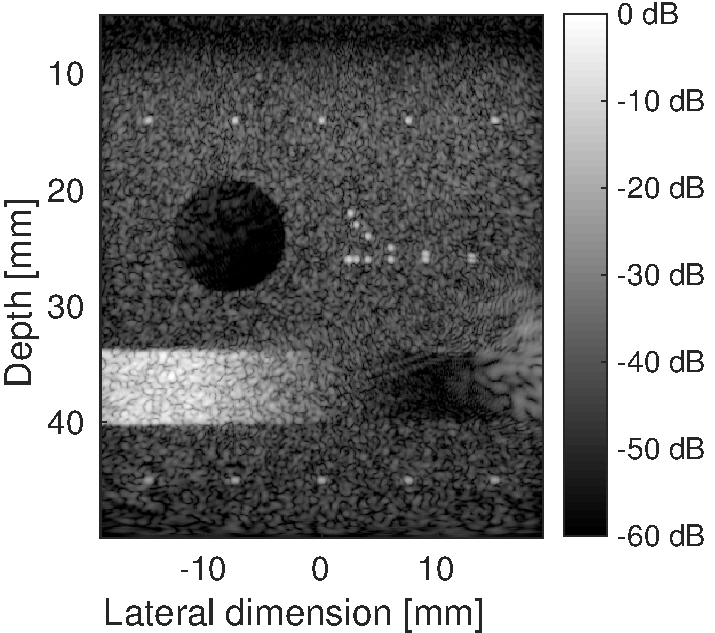
\includegraphics[width=\CohSubFigWidth]{Figures/das_dataset_rf_numerical_transmission_1_nbPW_1.pdf}}
\begin{figure}[htb]
	% Maximum length
	\hfill%
	\subcaptionbox{\label{fig_numerical_DAS}}{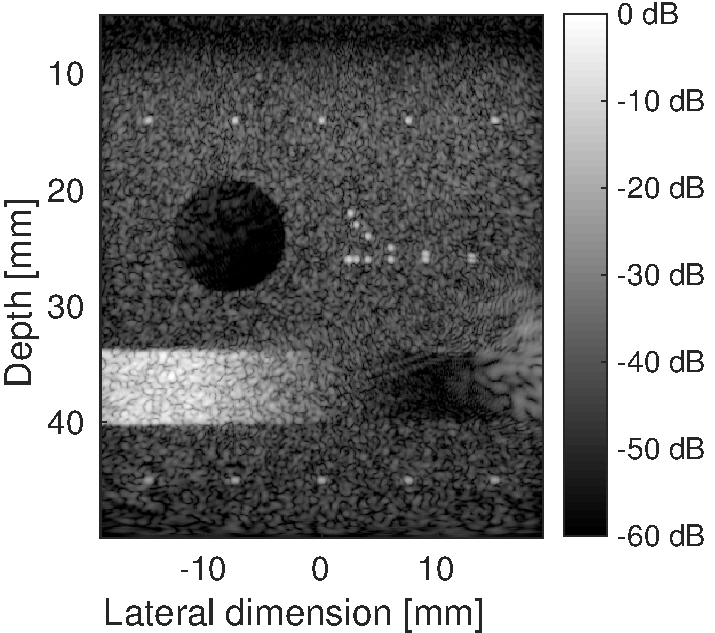
\includegraphics[height=\CohSubFigHeight]{Figures/das_dataset_rf_numerical_transmission_1_nbPW_1.pdf}}\hfill%
	\subcaptionbox{\label{fig_numerical_DAS_5}}{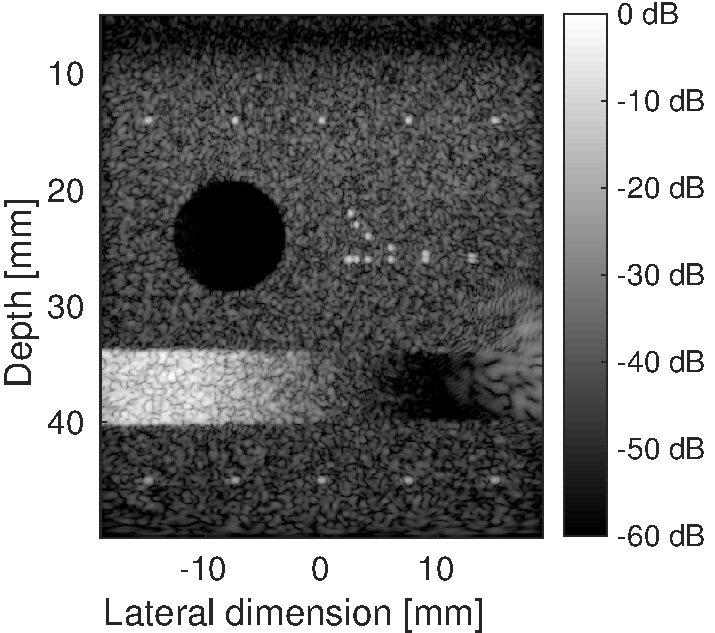
\includegraphics[height=\CohSubFigHeight]{Figures/das_dataset_rf_numerical_transmission_1_nbPW_5.pdf}}\hfill%
	\subcaptionbox{\label{fig_numerical_FISTA}}{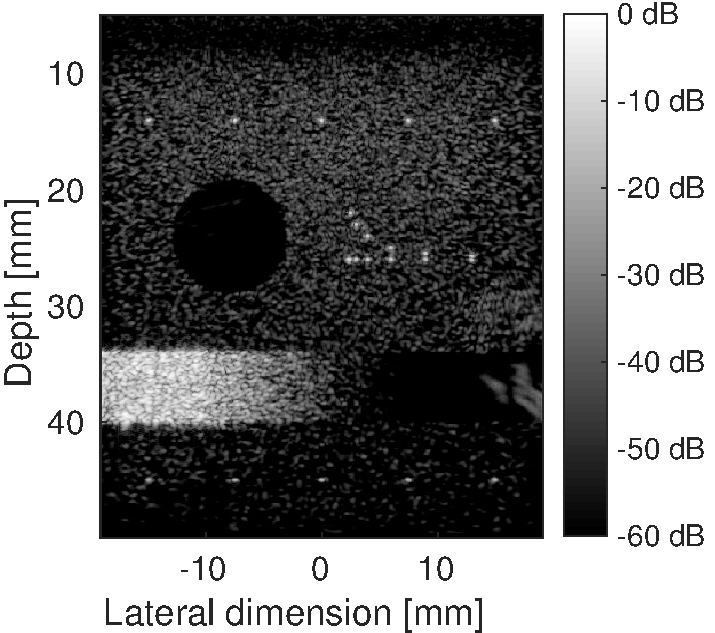
\includegraphics[height=\CohSubFigHeight]{Figures/FISTA_dataset_rf_numerical_transmission_1_nbPW_1.pdf}}\hfill%
	\subcaptionbox{\label{fig_numerical_FISTALP}}{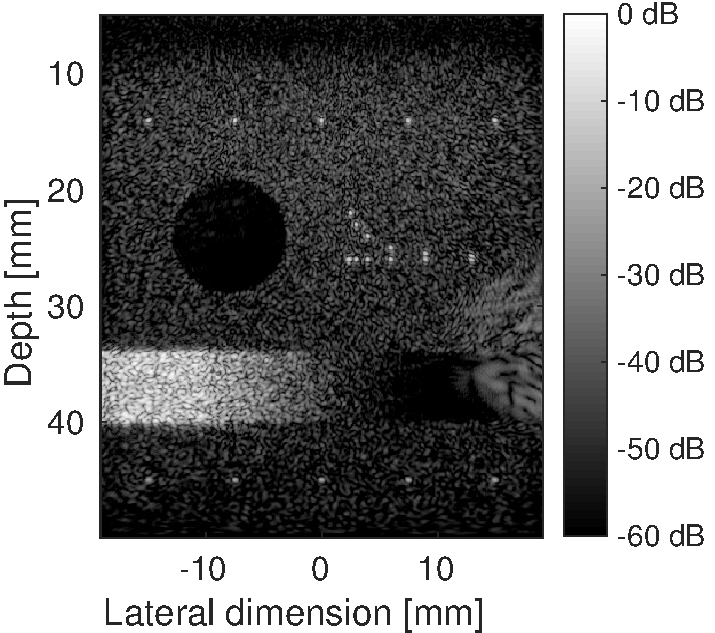
\includegraphics[height=\CohSubFigHeight]{Figures/FISTALP_dataset_rf_numerical_transmission_1_nbPW_1.pdf}}\hfill\null%
	
	\hfill%
	\subcaptionbox{\label{fig_carotid_DAS}}{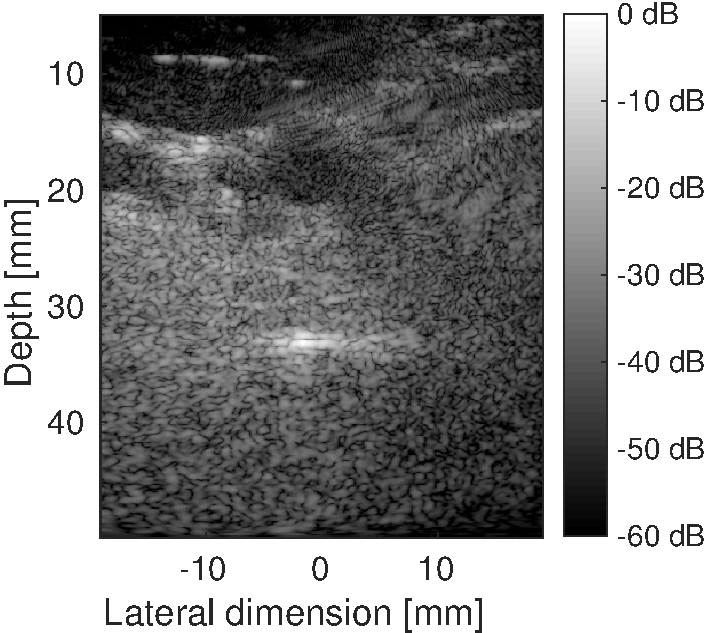
\includegraphics[height=\CohSubFigHeight]{Figures/das_carotid_cross_expe_dataset_rf.pdf}}\hfill%
	\subcaptionbox{\label{fig_carotid_DAS_5}}{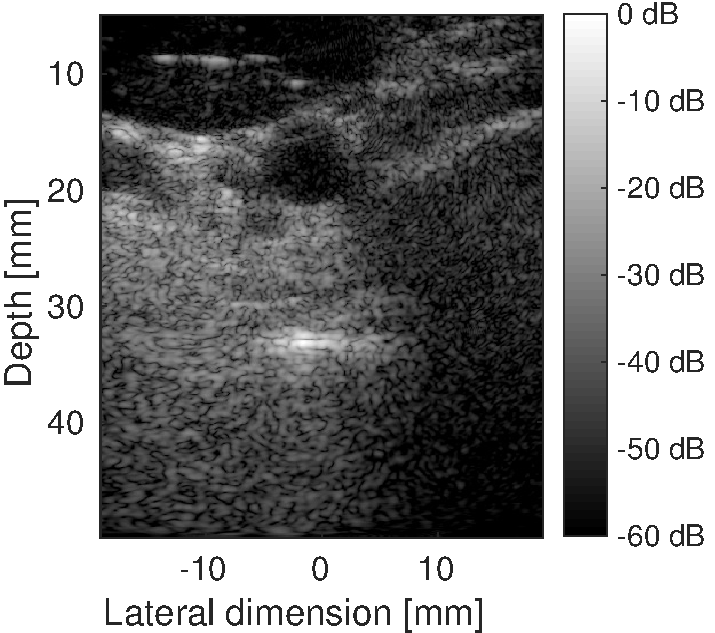
\includegraphics[height=\CohSubFigHeight]{Figures/das_carotid_cross_expe_dataset_rf_5PWs.pdf}}\hfill%
	\subcaptionbox{\label{fig_carotid_FISTA}}{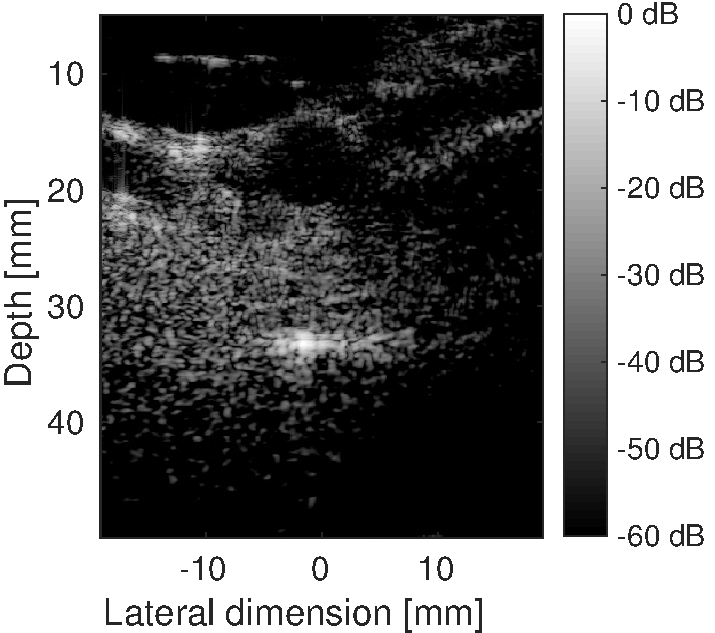
\includegraphics[height=\CohSubFigHeight]{Figures/FISTA_carotid_cross_expe_dataset_rf.pdf}}\hfill%
	\subcaptionbox{\label{fig_carotid_FISTALP}}{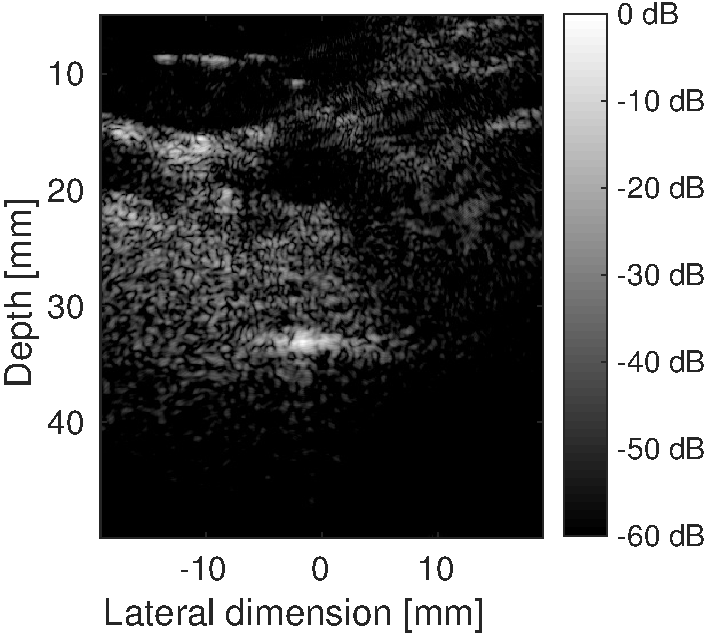
\includegraphics[height=\CohSubFigHeight]{Figures/FISTALP_carotid_cross_expe_dataset_rf.pdf}}\hfill\null%
	\caption{Image of the numerical phantom reconstructed with (a) DAS - 1 PW insonification, (b) DAS - 5 PW insonifications, (c) USSR-SA - 1 PW insonification, (c) USSR - $\ell_p$ - 1 PW insonification; Image of the \textit{in-vivo} carotid reconstructed with (e) DAS - 1 PW insonification, (f) DAS - 5 PW insonifications, (g) USSR-SA - 1 PW insonification, (h) USSR-$\ell_p$ - 1 PW insonification.}
	\label{fig_Bmode}
\end{figure}
	
\end{block}
\vfill

%----------------------------------------------------------------------------------------
%	CONCLUSION
%----------------------------------------------------------------------------------------
\begin{block}{Conclusion and perspectives}
	\begin{enumerate}
		\item We propose a compressed sensing approach for US image recovery
		\begin{itemize}
			\item Exploits a stream of pulses model for sparsity of US images
			\item Uses multiple CMUX for analog compression of the data
			\item Applies a $\ell_{11}$-minimization algorithm for image reconstruction
		\end{itemize}
		\item The proposed approach leads to high-quality reconstruction with far fewer data than standard approaches
		\item Study of the hardware implementation will be achieved in future work
	\end{enumerate}
\end{block}
\vfill
%----------------------------------------------------------------------------------------
%	BIBLIOGRAPHY
%----------------------------------------------------------------------------------------
\begin{block}{References}
	\printbibliography
\end{block}
\vfill
%----------------------------------------------------------------------------------------
%	ACKNOWLEDGMENTS
%----------------------------------------------------------------------------------------
\begin{block}{Acknowledgments}
	This work was supported in part by the UltrasoundToGo RTD project (no. 20NA21 145911), evaluated by the Swiss NSF and funded by Nano-Tera.ch with Swiss Confederation financing.
\end{block}
}%